\documentclass[10pt]{article}
\usepackage{icmlko}

\icmlmeta{IP 파운데이션 월드모델}{55}{예외에는 조건이 있었다}{여섯 도메인에 고유 축을 다 붙여 보니 게임만 좋아진다 --- 그리고 그 예외를 가르는 경계가 하나다}

\begin{document}

\twocolumn[
\icmlheader

\begin{abstract}
노트 54가 노트 36의 ``고유 축 확장은 소용없다''를 게임에 한해 정정했다. 그러면
다른 도메인은 어떤가. 자기 순위 상관이 가장 낮은 둘(도서 $+$0.202, 펀딩
$+$0.190)에 고유 축 후보를 새로 만들어 붙이고 여섯 도메인 전부를 쟀다.
\textbf{게임만 좋아진다}($+$0.0066). 나머지는 전부 나빠지고 웹툰이 $-$0.0474로
가장 크다. 왜 게임만인지 두 가지로 설명해 보았다 --- 기존 관측 축 수와 고유 축의
신호 강도. \textbf{둘 다 실패했다}(상관 $-$0.331과 $+$0.015). 그런데 축 수를
\emph{연속}이 아니라 \emph{경계}로 보면 완벽하게 갈린다. \textbf{관측 축이
둘인 게임만 양수이고 넷에서 다섯인 나머지는 전부 음수다.} 성분을 둘 뽑으므로,
축이 둘이면 인자 공간이 사실상 회전만 하고 넷 이상이면 이미 압축이 일어난다.
압축이 일어난 뒤에 축을 더하면 공통 축의 적재가 희석될 뿐이다 --- 노트 36이
관찰했던 그대로다. 조합해서 붙이면 나빠지는 것이 쌓인다($-$0.0629). 노트 36의
결론을 \textbf{대부분 복원하고 조건을 붙인다} --- 고유 축은 관측 축이 성분 수와
같을 때만 도움이 된다.
\end{abstract}
]

\section{여섯 도메인 전부에 붙여 봤다}

노트 54가 게임에서만 고유 축이 값을 한다는 것을 보였다. 도서와 펀딩은 자기
순위 상관이 각각 $+$0.202와 $+$0.190으로 가장 낮으니 얻을 것이 많아야 한다.
고유 축 후보를 새로 만들었다 --- 펀딩은 최고 후원가 · 배송 리워드 비율 · 성인
전용, 웹툰은 연령 등급 · 태그 수 · 회차 수 · 요일 수.

\begin{table}[t]
\centering\tsize
\caption{고유 축을 더할 때. 현행 $\rho=+0.3440$.}
\begin{tabular}{lrrrr}
\toprule
도메인 & 기존 축 & 고유 축 & 고유 축 $|r|$ & $\Delta\rho$ \\
\midrule
\textbf{게임} & \textbf{2} & 4 & 0.195 & \textbf{$+$0.0066} \\
도서 & 4 & 2 & 0.057 & $-$0.0017 \\
아이돌 & 5 & 3 & 0.063 & $-$0.0054 \\
팝업 & 5 & 5 & 0.089 & $-$0.0167 \\
펀딩 & 4 & 3 & 0.108 & $-$0.0256 \\
웹툰 & 4 & 4 & 0.131 & $-$0.0474 \\
\bottomrule
\end{tabular}
\end{table}

게임만 좋아진다.

\section{두 설명이 실패했다}

\begin{table}[t]
\centering\tsize
\caption{$\Delta\rho$를 무엇이 설명하나(여섯 점).}
\begin{tabular}{lr}
\toprule
후보 & 상관 \\
\midrule
기존 관측 축 수 & $-$0.331 \\
고유 축의 평균 $|r|$ & $+$0.015 \\
\bottomrule
\end{tabular}
\end{table}

축 수는 부호가 맞지만 약하고, 고유 축의 신호 강도는 아예 무관하다. 웹툰은 고유
축 신호가 0.131로 게임 다음인데 가장 크게 나빠진다.

\section{경계로 보면 갈린다}

\begin{figure}[t]
\centering
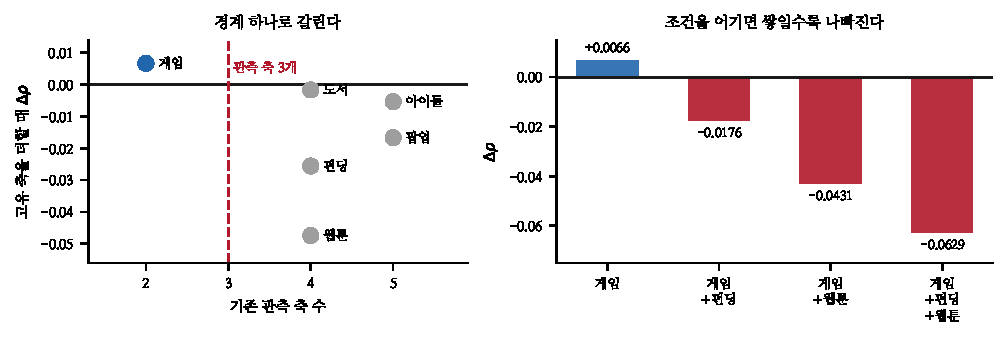
\includegraphics[width=\textwidth]{figs/owncond.pdf}
\caption{왼쪽 --- 기존 축 수와 효과. 오른쪽 --- 조건을 어긴 조합.}
\end{figure}

축 수를 연속 변수로 보지 말고 경계로 보면 완벽하게 갈린다.

\begin{quote}\fontsize{9.5}{11.5}\selectfont
\textbf{관측 축이 둘인 도메인만 양수이고, 넷에서 다섯인 도메인은 전부 음수다.}
경계가 셋 근처에 있고 여섯 점이 그것을 어기지 않는다.
\end{quote}

\claimx{고유 축은 관측 축 수가 성분 수(둘)와 같을 때만 도움이 된다. 축이 둘이면
주성분 분석이 사실상 회전만 하므로 더할 여지가 있고, 넷 이상이면 이미 압축이
일어난 뒤라 추가 축은 공통 축의 적재를 희석할 뿐이다.}{관측 축이 셋인 도메인이
나오면 경계를 직접 확인할 수 있다. 지금은 둘과 넷 사이가 비어 있어 경계 위치를
모른다.}

노트 36이 관찰한 것이 바로 이 희석이었다 --- 그 노트는 팝업에 고유 축 다섯을
더하면 2차원 통과율이 1.04에서 1.50으로 튀고 아이돌은 1.01에서 0.83으로 샌다고
적었다. 설명이 없었을 뿐 현상은 같다.

\paragraph{조건을 어기면 쌓인다}
\begin{table}[t]
\centering\tsize
\caption{조합해서 붙일 때.}
\begin{tabular}{lr}
\toprule
& $\Delta\rho$ \\
\midrule
게임 & $+$0.0066 \\
게임 $+$ 펀딩 & $-$0.0176 \\
게임 $+$ 웹툰 & $-$0.0431 \\
게임 $+$ 펀딩 $+$ 웹툰 & $-$0.0629 \\
\bottomrule
\end{tabular}
\end{table}

조건을 어긴 도메인을 더할수록 손해가 쌓인다. 게임의 이득이 하나만 붙였을 때
살아 있고 둘을 더하는 순간 잠긴다.

\section{노트 36을 어떻게 정리하나}

\begin{itemize}[leftmargin=1.1em,itemsep=0.2em]
\item \textbf{복원} --- ``고유 축을 늘리면 대체로 나빠진다.'' 여섯 도메인 중
      다섯에서 그렇다.
\item \textbf{조건 추가} --- 관측 축이 성분 수와 같은 도메인은 예외다. 지금은
      게임 하나뿐이다.
\item \textbf{철회 유지} --- 노트 36의 ``상한이 두 개''는 노트 37에서 이미
      기각됐고 여기서 바뀌지 않는다.
\end{itemize}

이 조건은 설계 규칙으로 쓸 수 있다. \textbf{새 도메인을 넣을 때 관측 축이
둘이면 고유 축을 찾고, 넷 이상이면 찾지 않는다.} 지금까지는 도메인마다 시험해
봐야 알았다.

\section{한계}

\begin{itemize}[leftmargin=1.1em,itemsep=0.15em]
\item 관측 축이 셋인 도메인이 없어 경계 위치를 모른다. 둘과 넷 사이 어디든 될
      수 있다.
\item 여섯 점으로 경계를 그었다. 게임이 유일한 양수이므로 그 한 점이 전부를
      떠받친다.
\item 각 도메인의 고유 축 후보를 내가 골랐다. 더 좋은 후보가 있으면 부호가
      바뀔 수 있다 --- 특히 도서(고유 축 $|r|$ 0.057)는 후보가 빈약하다.
\item 성분 수를 둘로 고정한 채 봤다. 성분을 셋으로 늘리면 경계도 옮겨갈 것이며,
      그것은 공통 축 수에 묶여 있다(노트 37).
\item 짝지은 구간을 게임에만 붙였다. 나머지 다섯의 음수가 잡음인지 확인하지 않았다.
\end{itemize}

\section{다음}

\begin{enumerate}[leftmargin=1.3em,itemsep=0.15em]
\item 관측 축이 셋인 도메인을 만들어 경계를 찾는다 --- 기존 도메인에서 축 하나를
      꺼 보면 된다.
\item 웹툰 전체 완결작 수집 --- 진행 중(959/3,973).
\item 도서 고유 축 후보를 늘린다. 지금은 쪽수와 무게뿐이다.
\item 다섯 도메인의 음수에 구간을 붙인다.
\end{enumerate}

\vspace{0.6em}
\hrule height 0.3pt
\vspace{0.5em}
{\footnotesize
\textbf{참고문헌}\\[0.3em]
Jolliffe, I. T. (2002). \emph{Principal Component Analysis}, 2nd ed. Springer.\\[0.15em]
Schönemann, P. H. (1966). A generalized solution of the orthogonal Procrustes
problem. \emph{Psychometrika}, 31(1), 1--10.\\[0.15em]
Meredith, W. (1993). Measurement invariance, factor analysis and factorial
invariance. \emph{Psychometrika}, 58(4), 525--543.\\[0.15em]
Efron, B., Tibshirani, R. J. (1993). \emph{An Introduction to the Bootstrap}.
Chapman \& Hall.\\[0.15em]
Ben-David, S. et al. (2010). A theory of learning from different domains.
\emph{Machine Learning}, 79(1--2), 151--175.
}

\end{document}
